\documentclass{article}
\usepackage[paperwidth=12in,paperheight=7in,margin=0.25in]{geometry}
\usepackage{tikz}
\usetikzlibrary{arrows.meta,positioning,shapes.geometric}
\pagestyle{empty}

\begin{document}
\centering
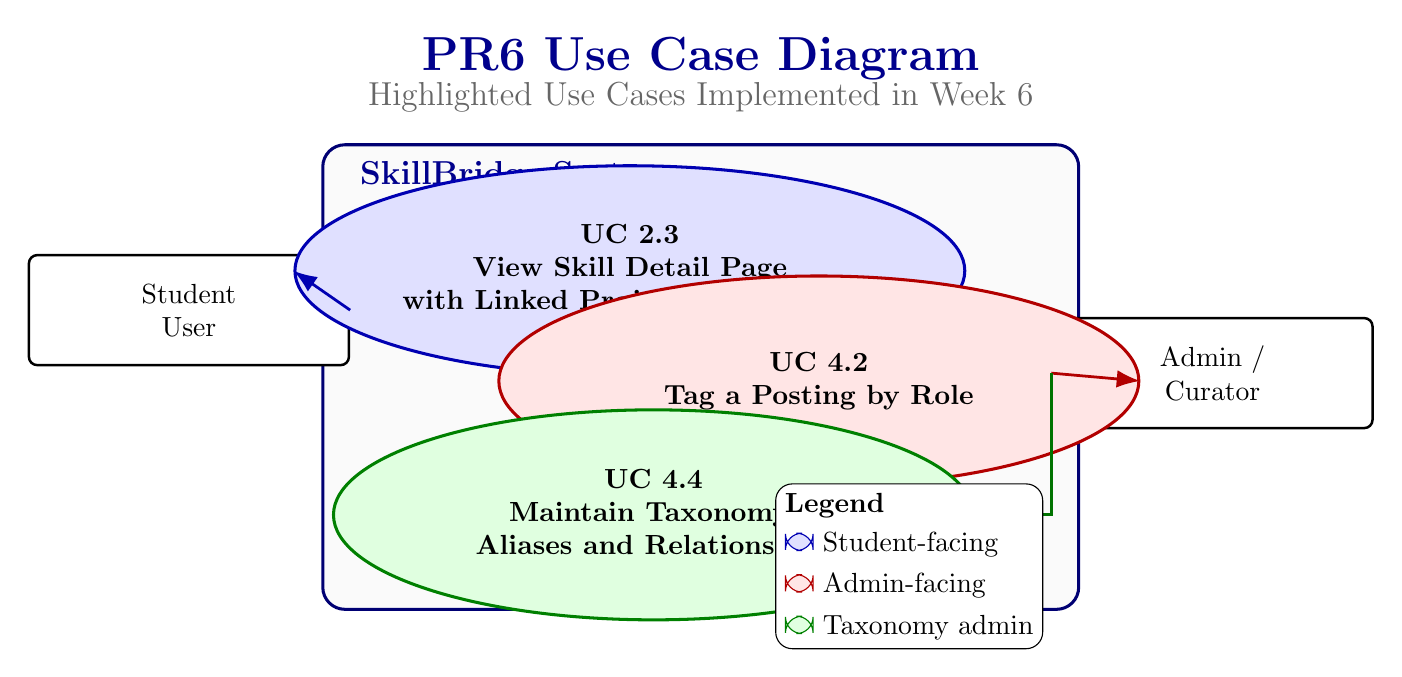
\begin{tikzpicture}[
  actor/.style={draw, line width=0.9pt, fill=white, minimum width=1.6in, minimum height=0.55in, rounded corners=3pt, align=center},
  usecase/.style={ellipse, draw, line width=1.1pt, minimum width=3.2in, minimum height=1.05in, align=center, font=\bfseries},
  studentuc/.style={usecase, fill=blue!12, draw=blue!70!black},
  adminuc/.style={usecase, fill=red!10, draw=red!70!black},
  taxonomyuc/.style={usecase, fill=green!12, draw=green!50!black},
  connector/.style={line width=1.0pt, -{Latex[length=3mm]}}
]

\node[font=\bfseries\LARGE, text=blue!55!black] at (0, 4.1) {PR6 Use Case Diagram};
\node[font=\large, text=black!60] at (0, 3.6) {Highlighted Use Cases Implemented in Week 6};

\draw[rounded corners=8pt, line width=1.1pt, fill=black!2, draw=blue!45!black] (-4.8,-2.9) rectangle (4.8,3.0);
\node[anchor=west, font=\bfseries\large, text=blue!55!black] at (-4.45,2.6) {SkillBridge System};

\node[actor] (student) at (-6.5,0.9) {Student\\User};
\node[actor] (admin) at (6.5,0.1) {Admin /\\Curator};

\node[studentuc] (uc23) at (-0.9,1.4) {UC 2.3\\View Skill Detail Page\\with Linked Projects / Evidence};
\node[adminuc] (uc42) at (1.5,0.0) {UC 4.2\\Tag a Posting by Role};
\node[taxonomyuc] (uc44) at (-0.6,-1.7) {UC 4.4\\Maintain Taxonomy:\\Aliases and Relationships};

\draw[connector, blue!70!black] (student.east) -- (uc23.west);
\draw[connector, red!70!black] (admin.west) -- (uc42.east);
\draw[connector, green!45!black] (admin.west) |- (uc44.east);

\node[draw, rounded corners=6pt, fill=white, align=left, anchor=north east] at (4.35,-1.3) {
  \textbf{Legend}\\[2pt]
  \tikz{\draw[fill=blue!12, draw=blue!70!black] (0,0) rectangle (0.35,0.22);} Student-facing\\[3pt]
  \tikz{\draw[fill=red!10, draw=red!70!black] (0,0) rectangle (0.35,0.22);} Admin-facing\\[3pt]
  \tikz{\draw[fill=green!12, draw=green!50!black] (0,0) rectangle (0.35,0.22);} Taxonomy admin
};

\end{tikzpicture}
\end{document}
